\mer{MER: Old, revisit to see if we have forgotten any of these interesting ideas.}
\subsection*{Effect of interfaces (interface permeability)}

\begin{itemize}
    \item Model 0 (baseline): only diffusion, different diffusion coefficient in the parenchyma and SAS/PVS. No leak to vasculature (zero permeability). $\infty$ $\zeta_0$ at the PVS-SAS interface, $\zeta_1$ at the PVS-SAS interface. Koch et al could be a reference for PVS-parenchyma, maybe Tithof et al (2022, "A network model" ...) could give some ideas for parameters, also see Mestre et al, Nature comms, 2022. 
    \item 
    With altered interface permeabilities in the PVS (Model 1), and or in the parenchyma (Model 2) 
    \end{itemize}


\subsection*{Effect of convection}
\begin{itemize}
    \item 
    With convective flow in the PVS (zero flow in the parenchyma for now)
    \begin{itemize}
        \item 
        Model 3: PVS flow equal to 18.7 $\mu$m/s
        \item 
        Model 4: Better PVS flow (distributed, according to conservation of mass, assumptions on PVS area)
    \end{itemize}    
    \item 
    With convective flow in the ECS (out of scope here, for follow-up work?)
\end{itemize}

\begin{figure}
    \centering
    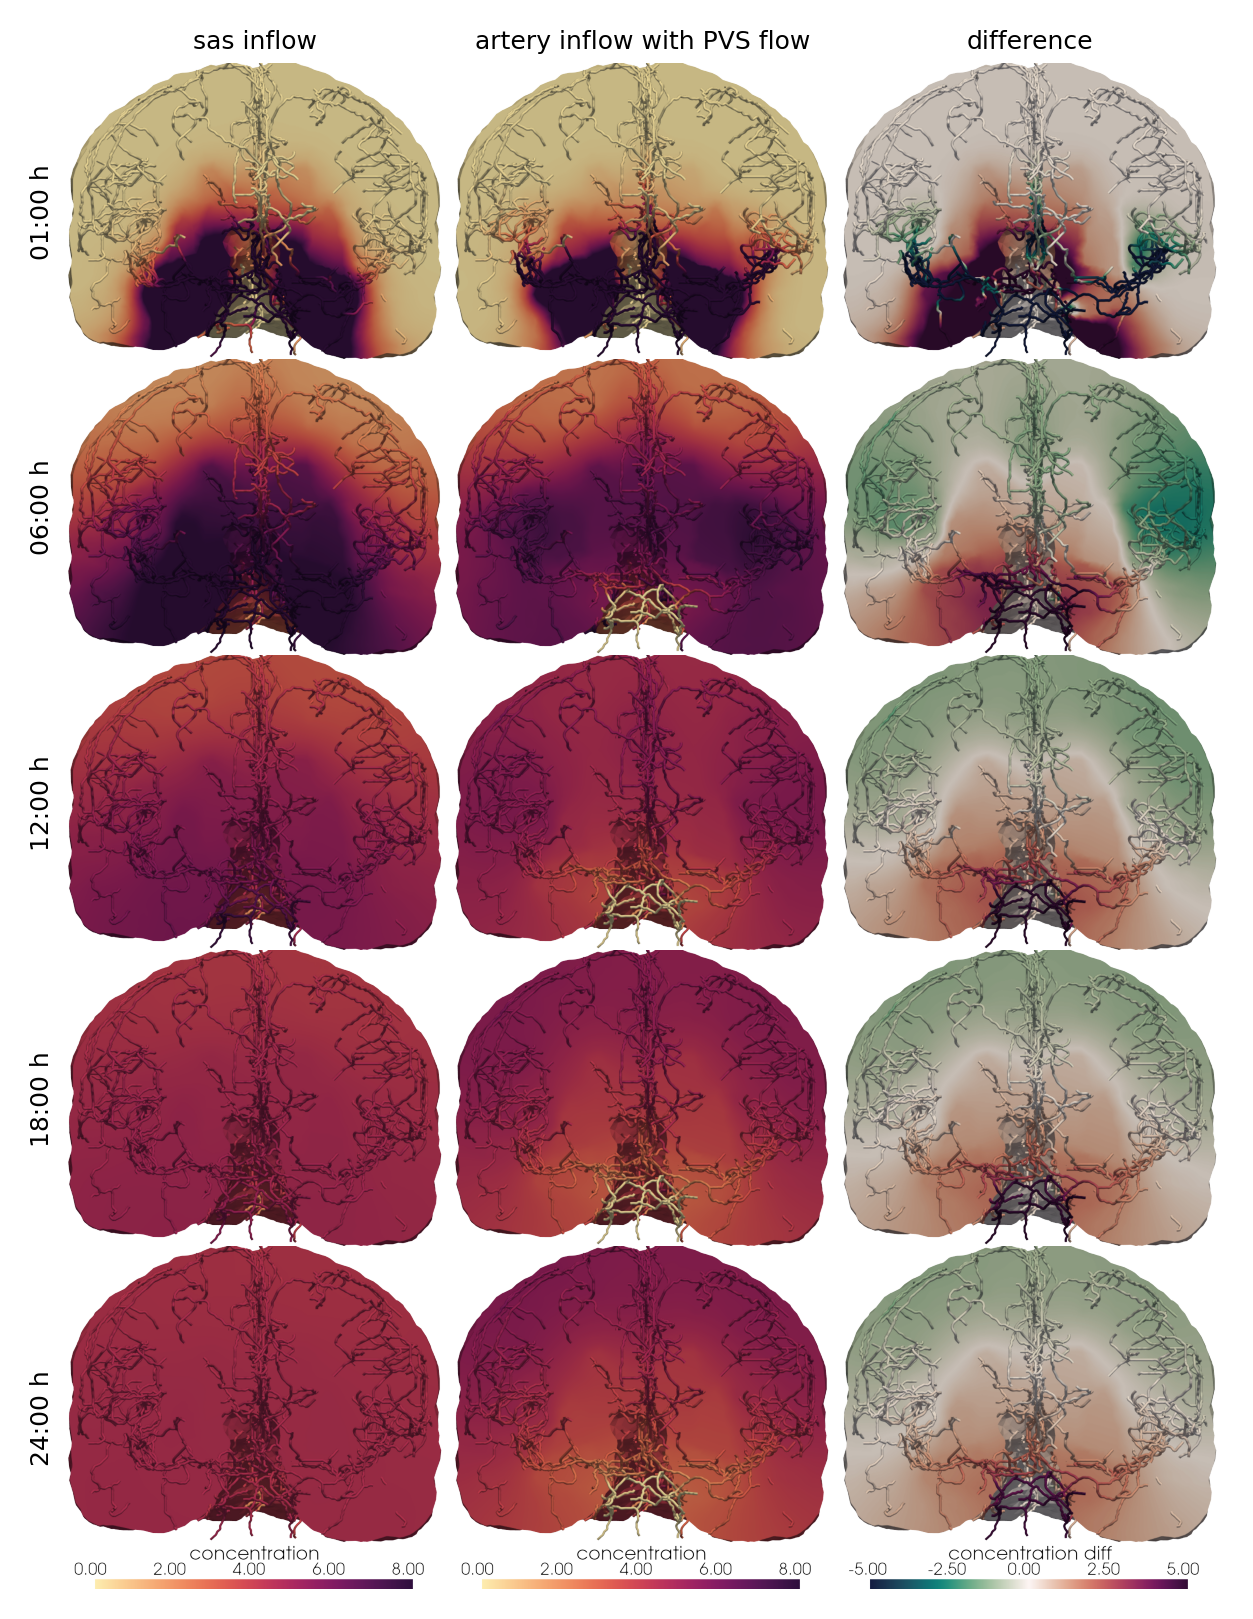
\includegraphics[width = 0.9 \textwidth]{modelB_modelC_overview.png}
    \caption{Tracer concentrations for a purely diffusive model with tracer inflow via the CSF-filled space (left) and a convective model with Tracer inflow via the arterial PVS (middle) and their difference (right) at 1, 6, 12, 18 and 24 hours after injection.}
    \label{fig:2}
\end{figure}

\subsection*{Effect of pia}
  
Effect of pia permeability (Model N-1)    

\begin{figure}
     \centering
     \begin{subfigure}[b]{0.33\textwidth}
         \centering
         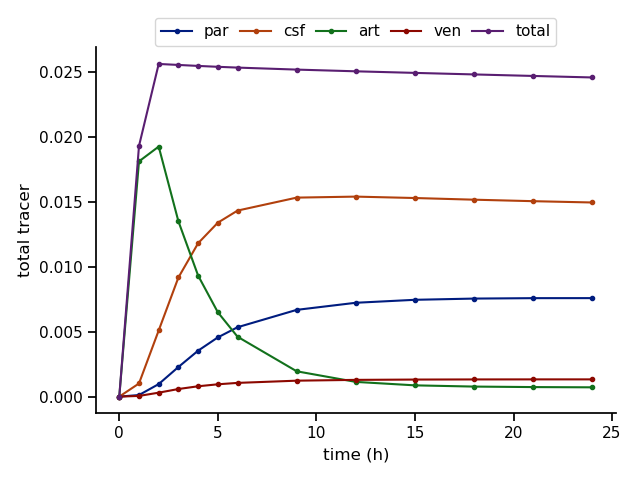
\includegraphics[width=\textwidth]{modelA_total_conc.png}
         \caption{arterial inflow, pure diffusion}
         \label{fig:y equals x}
     \end{subfigure}
     \hfill
     \begin{subfigure}[b]{0.33\textwidth}
         \centering
         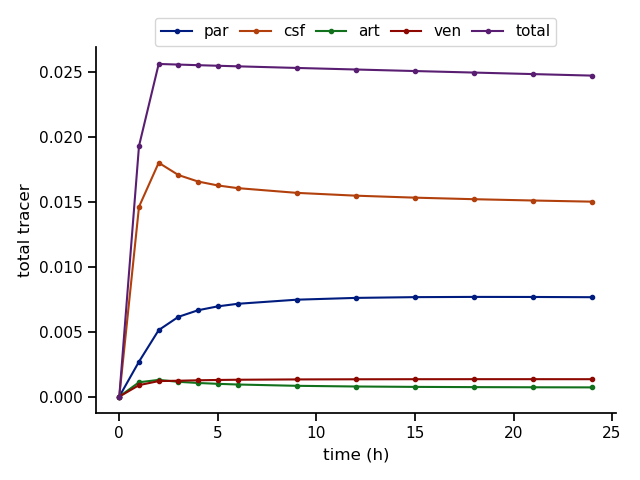
\includegraphics[width=\textwidth]{modelB_total_conc.png}
         \caption{SAS inflow, pure diffusion}
         \label{fig:three sin x}
     \end{subfigure}
     \hfill
     \begin{subfigure}[b]{0.33\textwidth}
         \centering
         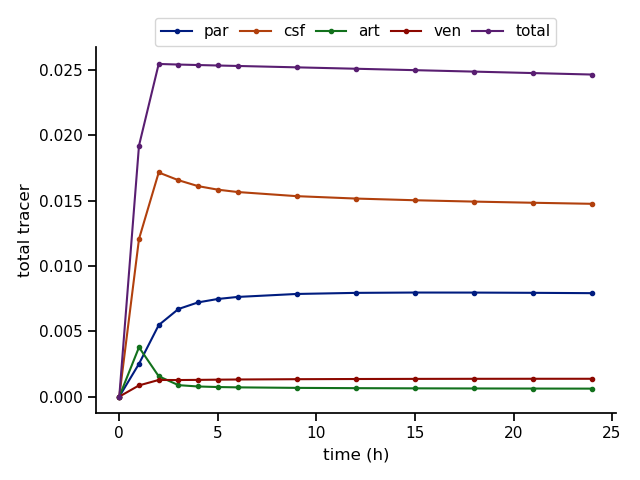
\includegraphics[width=\textwidth]{modelC_total_conc.png}
         \caption{arterial inflow, diffusion + PVS convection}
         \label{fig:five over x}
     \end{subfigure}
        \caption{Total tracer amount in parenchyma, CSF, arterial PVS and venous PVS}
        \label{fig:three graphs}
\end{figure}

\begin{figure}
\begin{subfigure}{0.5 \linewidth}
    \centering
    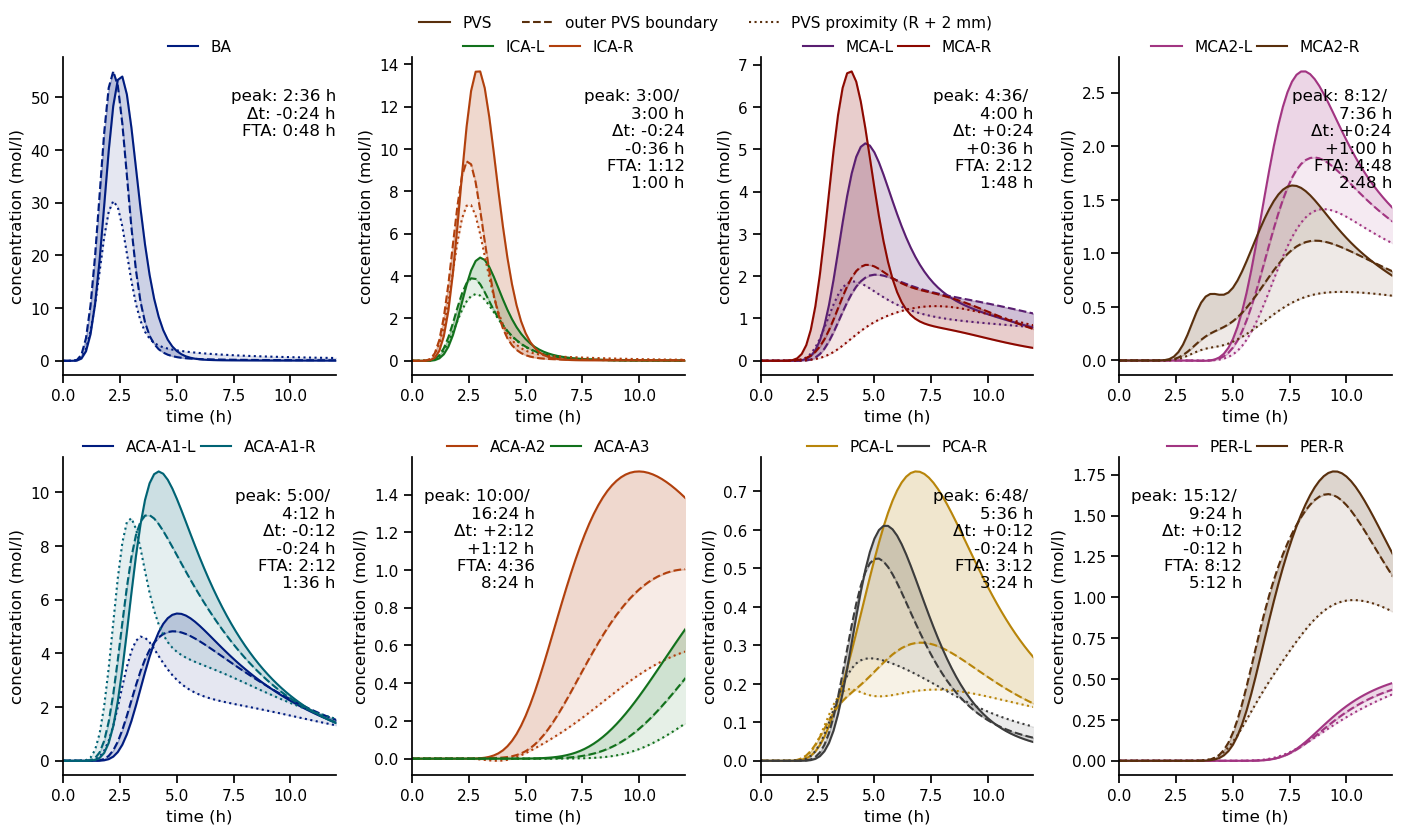
\includegraphics[width=1\linewidth]{figures/modelA_conc_at_label.png}
    \caption{B1 - $\xi$}
    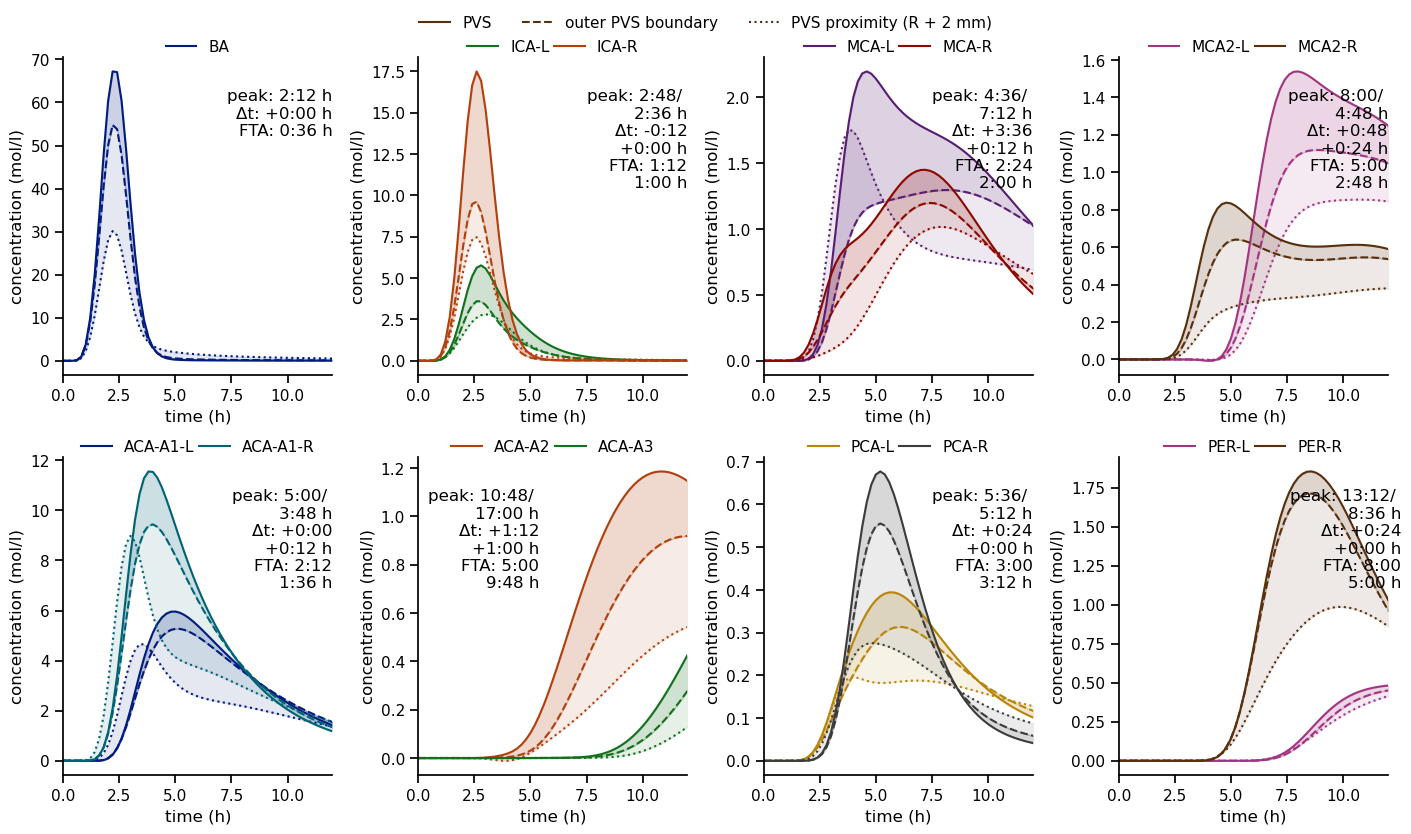
\includegraphics[width=1\linewidth]{figures/modelB1-10_conc_at_label.png}
    \caption{B1 - $10 \xi$}
    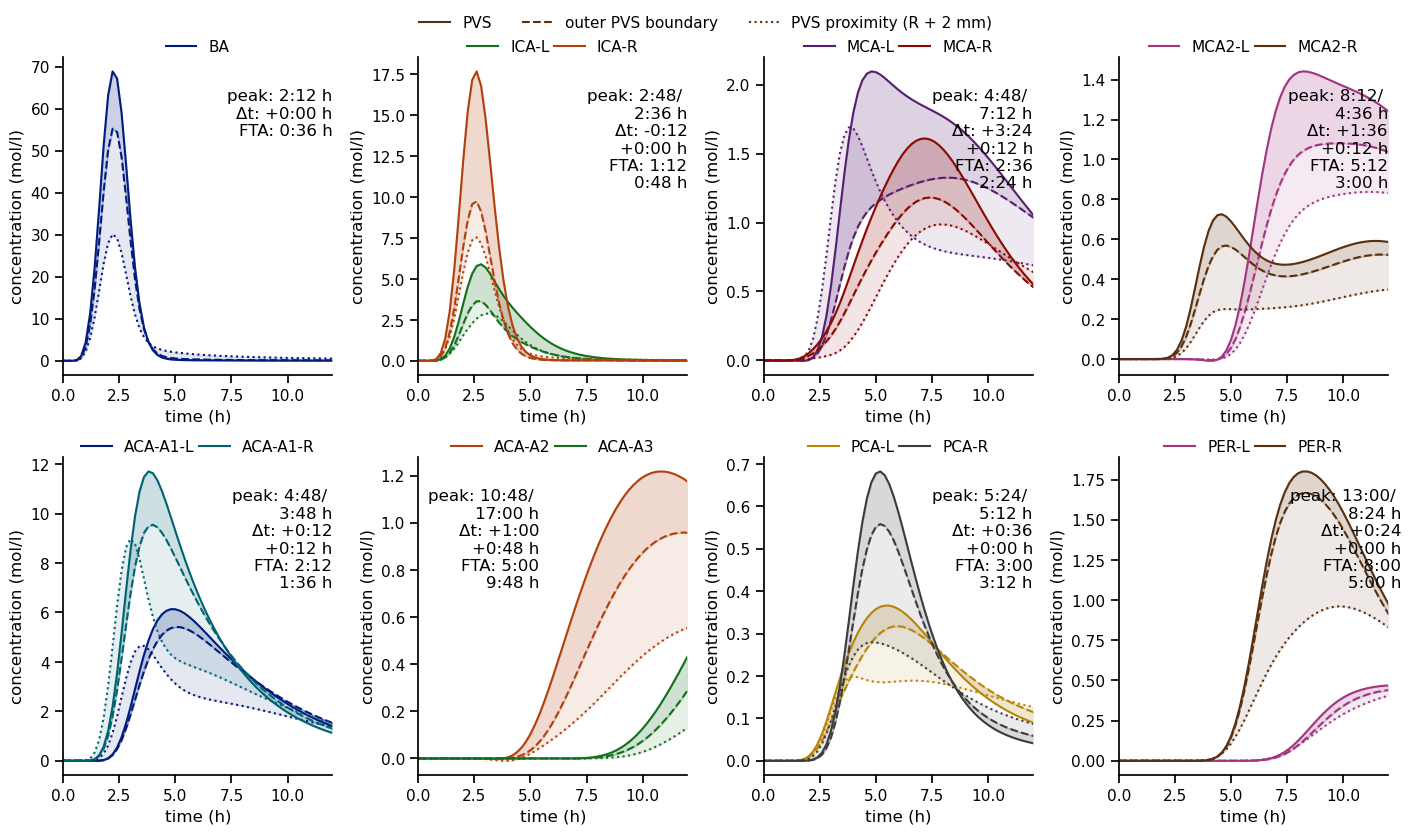
\includegraphics[width=1\linewidth]{figures/modelB1-100_conc_at_label.png}
    \caption{B1 - $100 \xi$}
    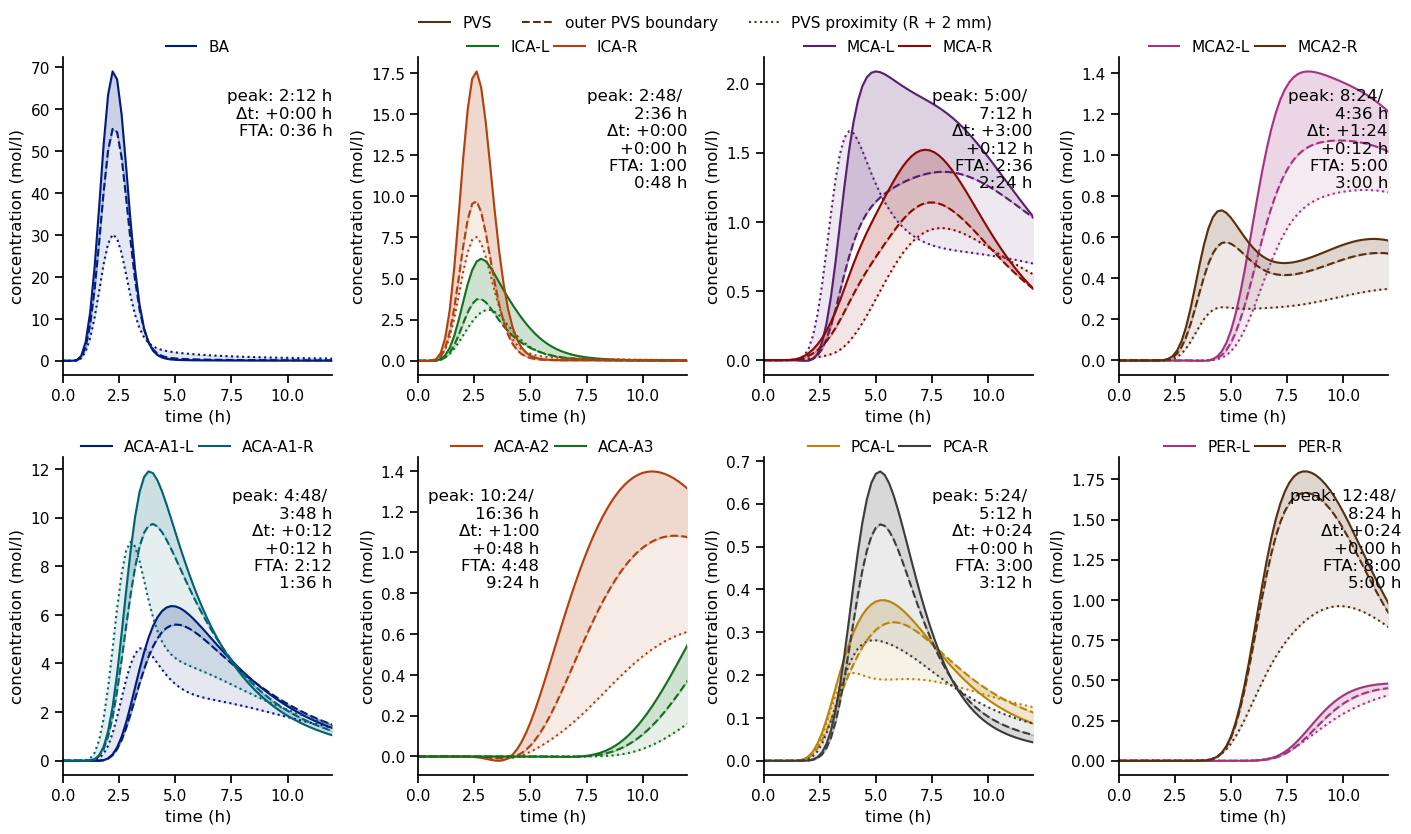
\includegraphics[width=1\linewidth]{figures/modelB1-1000_conc_at_label.png}
    \caption{B1 - $1000 \xi$}
\end{subfigure}
\begin{subfigure}{0.5 \linewidth}
    \centering
    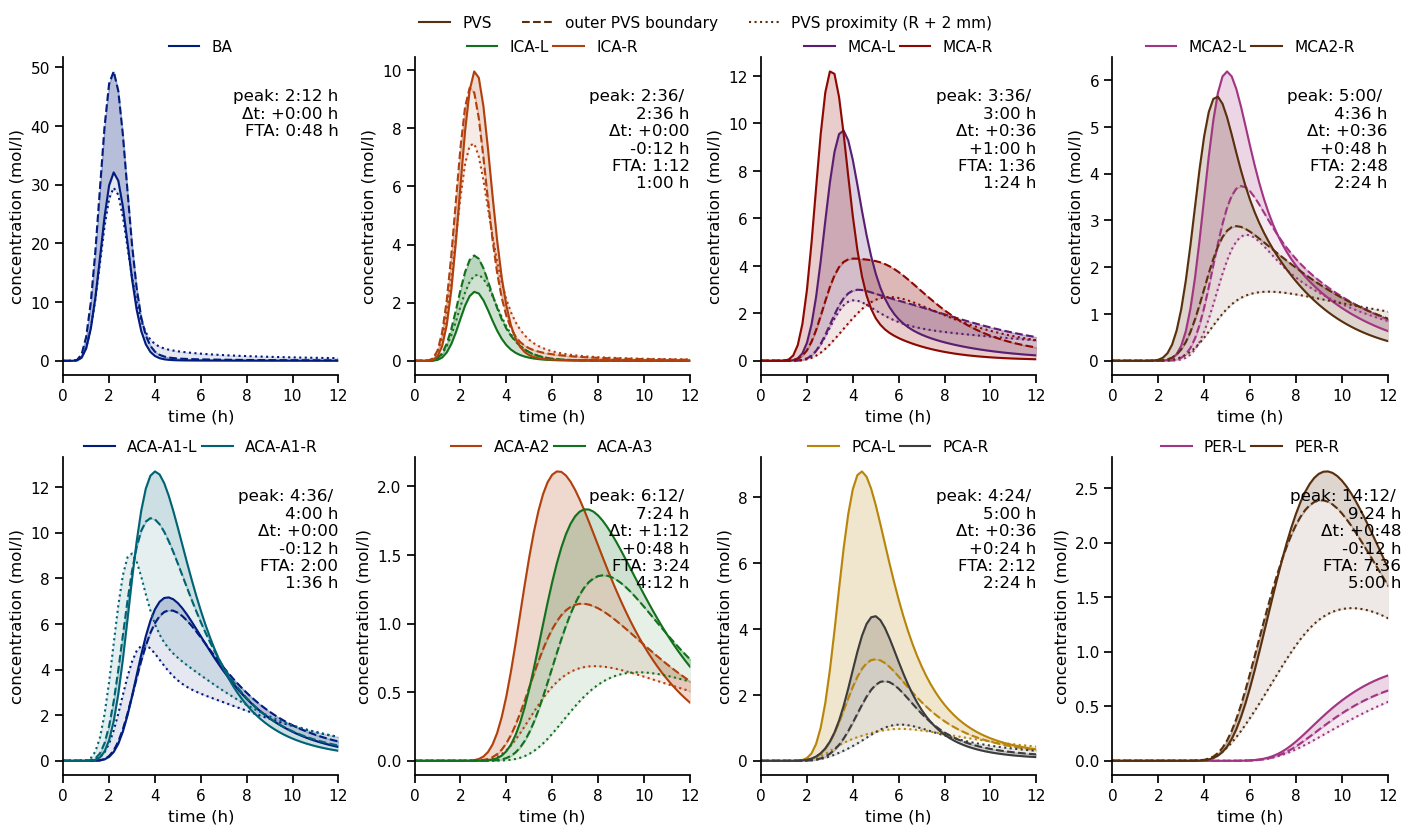
\includegraphics[width=1\linewidth]{figures/modelB2-1_conc_at_label.png}
    \caption{B2 - $\xi$}
    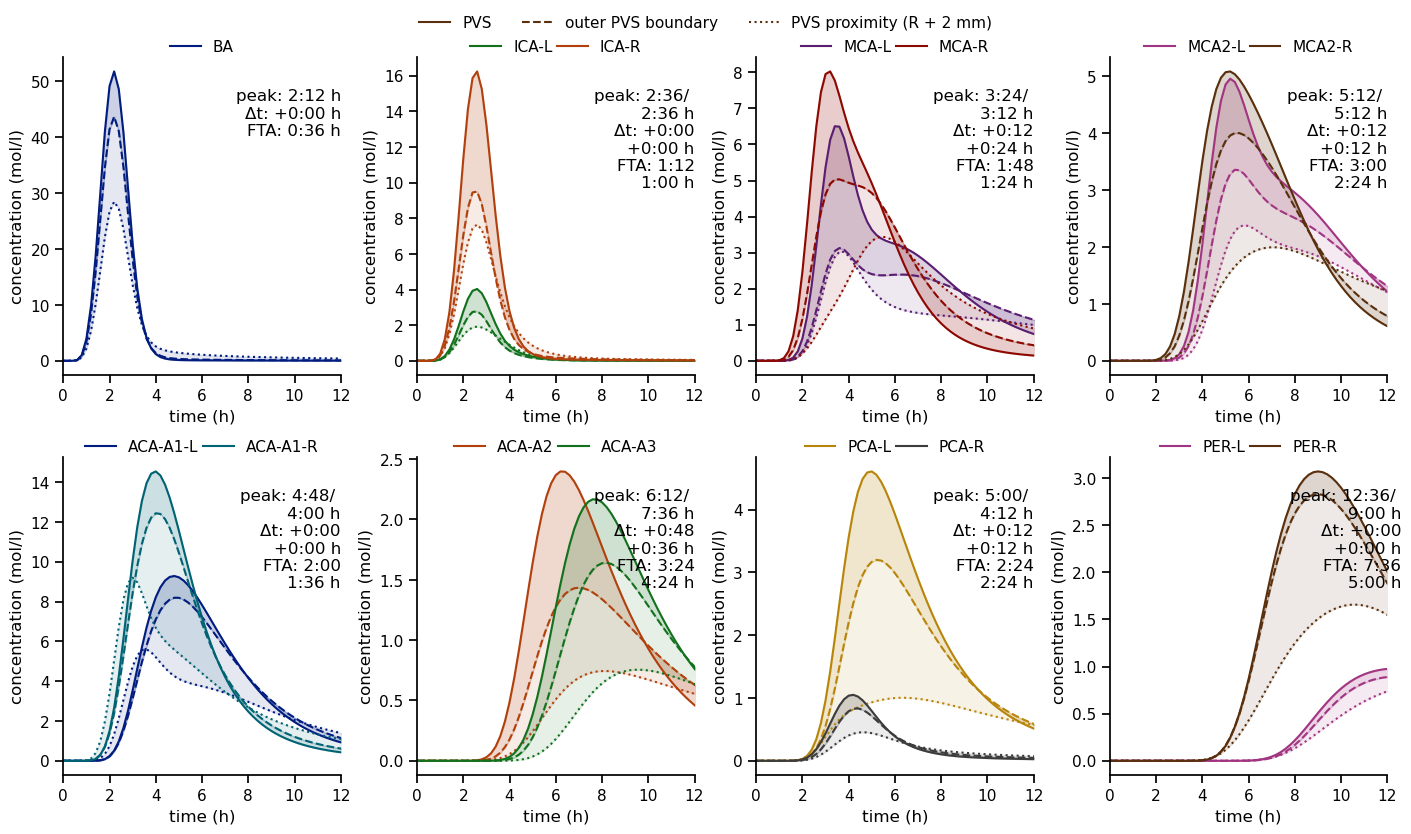
\includegraphics[width=1\linewidth]{figures/modelB2-10_conc_at_label.png}
    \caption{B2 - $10 \xi$}
    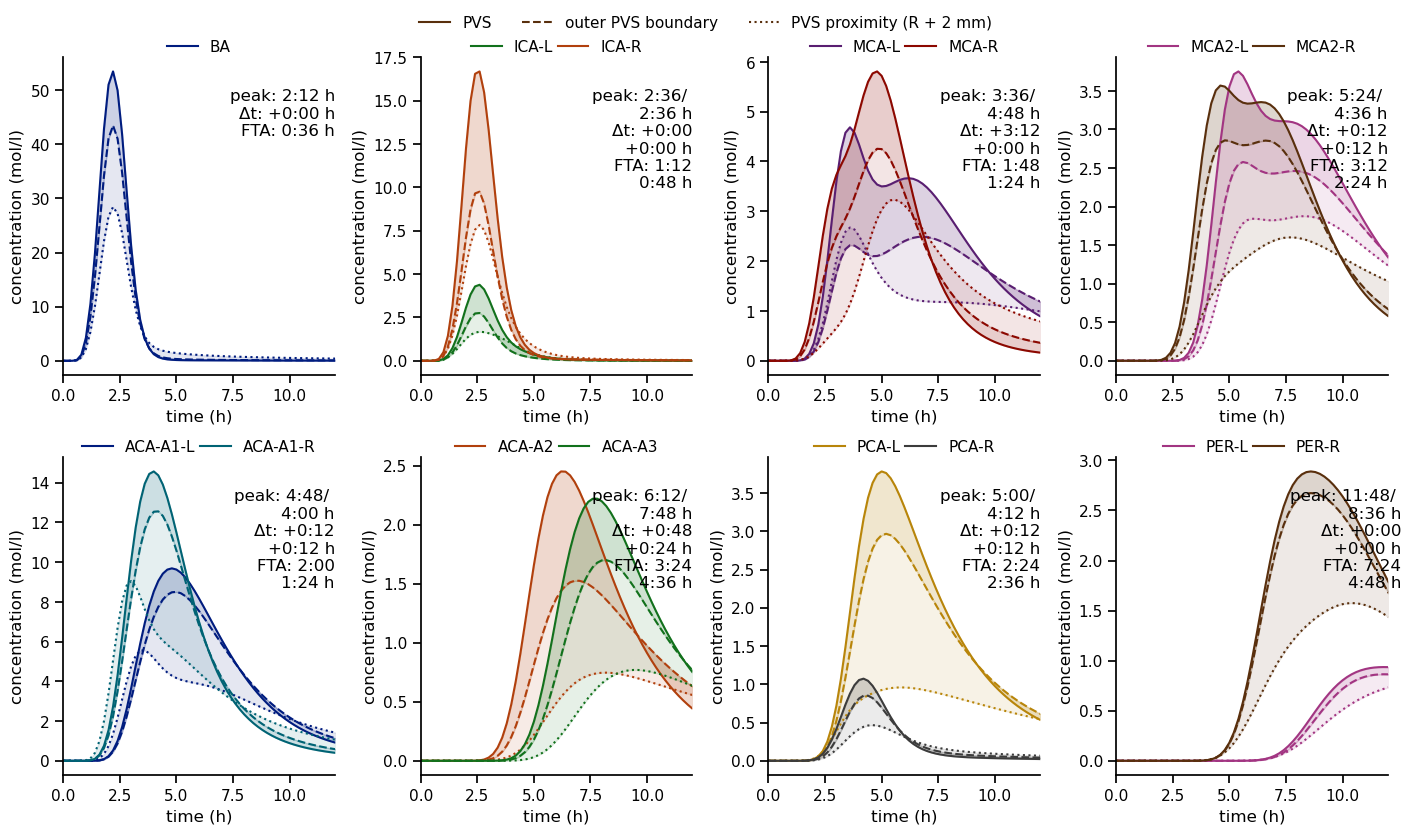
\includegraphics[width=1\linewidth]{figures/modelB2-100_conc_at_label.png}
    \caption{B2 - $100 \xi$}
    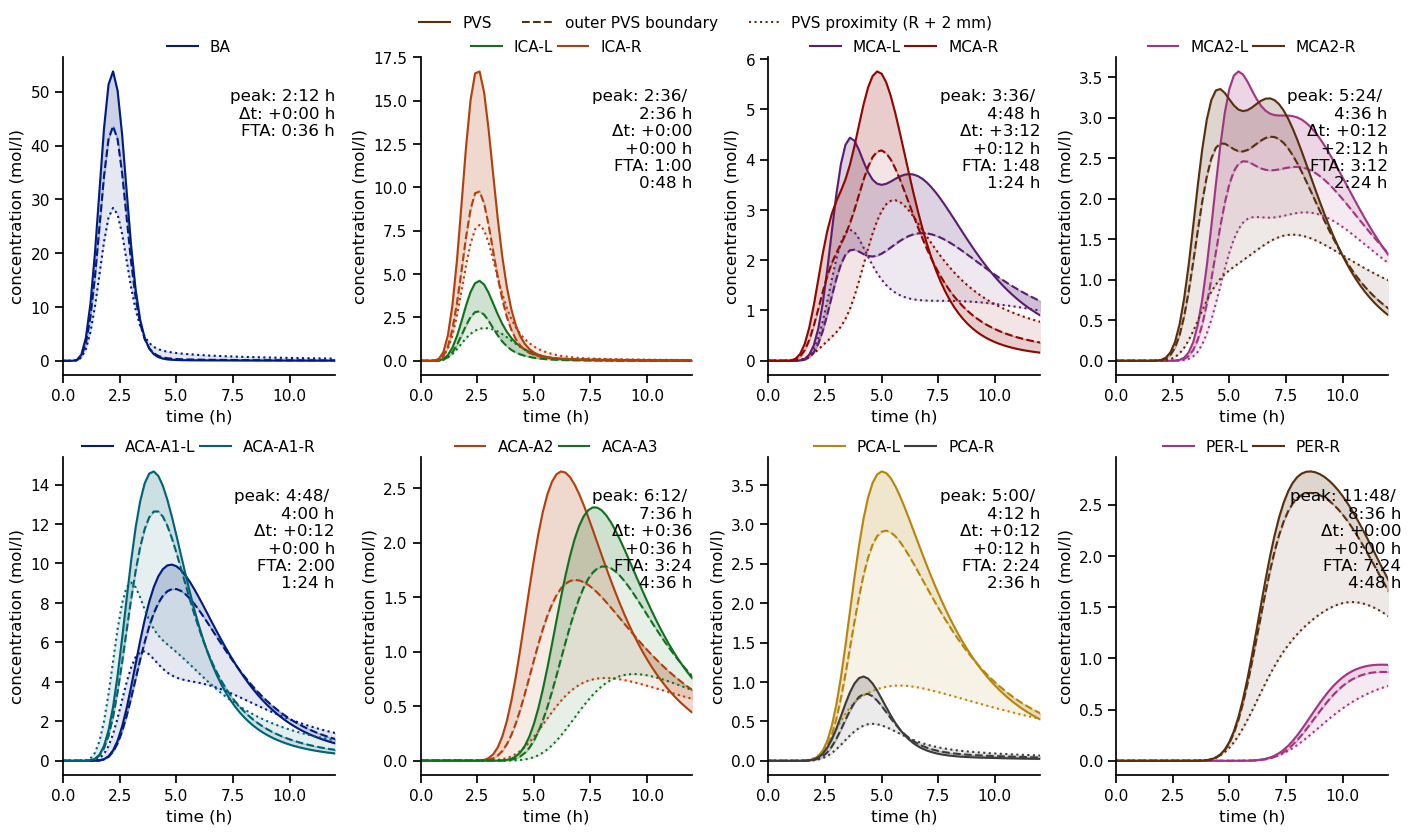
\includegraphics[width=1\linewidth]{figures/modelB2-1000_conc_at_label.png}
    \caption{B2 - $1000 \xi$}
\end{subfigure}
    \label{fig:modelB_xi_variations}
\end{figure}



\section{Foo}

We consider non-zero convection in the CSF space $u_{\rm CSF} \not = 0$ in \eqref{eq:multi_transport_3d} resulting from steady state CSF production.  Recall that $\Omega_{\mathrm{CSF}}$ represents the CSF space and that $\Gamma_{\mathrm{skull^{u/l}}}$ and $\Gamma_{\mathrm{pia}}$, $\Gamma_{\mathrm{LV}}$ represent the boundaries facing the upper and lower parts of the dura, the pia and the lateral ventricles, respectively.  Assuming CSF production in the choroid plexus located at the lateral ventricle wall, we solve the  steady state Stokes equations for the velocity and the pressure $(\bm u_{\mathrm{CSF}}, p_{\mathrm{CSF}})$ in the CSF domain: 
\begin{subequations}
    \begin{alignat}{2}
 - \mu \Delta \bm u_{\mathrm{CSF}} + \nabla p_{\rm{CSF}} & =  0 \quad && \mathrm{in} \,\,  \Omega_{\rm CSF}, \label{eq:momnetum_equation}  \\ 
 \nabla \cdot  \bm u_{\mathrm{CSF}} & = 0 \quad && \mathrm{in} \,\,   \Omega_{\rm CSF}, \label{eq:divergence_equation}  \\ 
\mu \nabla \bm u_{\mathrm{CSF}} \cdot \bm{n} -  p \bm n  &  = -R_0 ( \bm u \cdot \bm n ) \bm n\,\,   && \mathrm{on}  \label{eq:efflux_condition} \,\, \Gamma_{\mathrm{skull^u}}, \\ 
\bm u_{\mathrm{CSF}} & = 0 && \mathrm{on} \,\, \Gamma_{\rm{pia}} \cup \Gamma_{\mathrm{skull^l}} \Gamma_{\rm{SSAS}}  \\
\bm u_{\mathrm{CSF}} \cdot \bm n & = \frac{1}{ |\Gamma_{\rm LV}|}  u_{\rm in}, \quad \bm u \cdot \bm \tau = 0 \quad && \mathrm{on} \,\, \Gamma_{\rm{LV}} .  
\end{alignat}
\end{subequations}

Here, $\bm n$ denotes the unit outward normal to the boundary, $\mu$ is the CSF viscosity, and $\bm u_{\rm in}$ is the steady CSF flow across the lateral ventricle wall, see \Cref{tab:pvs:parameters}.
Condition \eqref{eq:efflux_condition} models an efflux site with positive resistance $R_0 \geq 0$. The Stokes system is solved with the finite element software $FEniCS$, stored and then subsequently read for all the relevant solute transport simulations. See Figure~\ref{fig:csf_flow_cardiac} for a streamline visualization of the obtained velocity profile and \Cref{sec:details_numerical_method} for details on the numerical algorithm employed.

%% \begin{figure}
%%      \centering
%%      \begin{subfigure}[b]{0.45\textwidth}
%%          \centering
%%          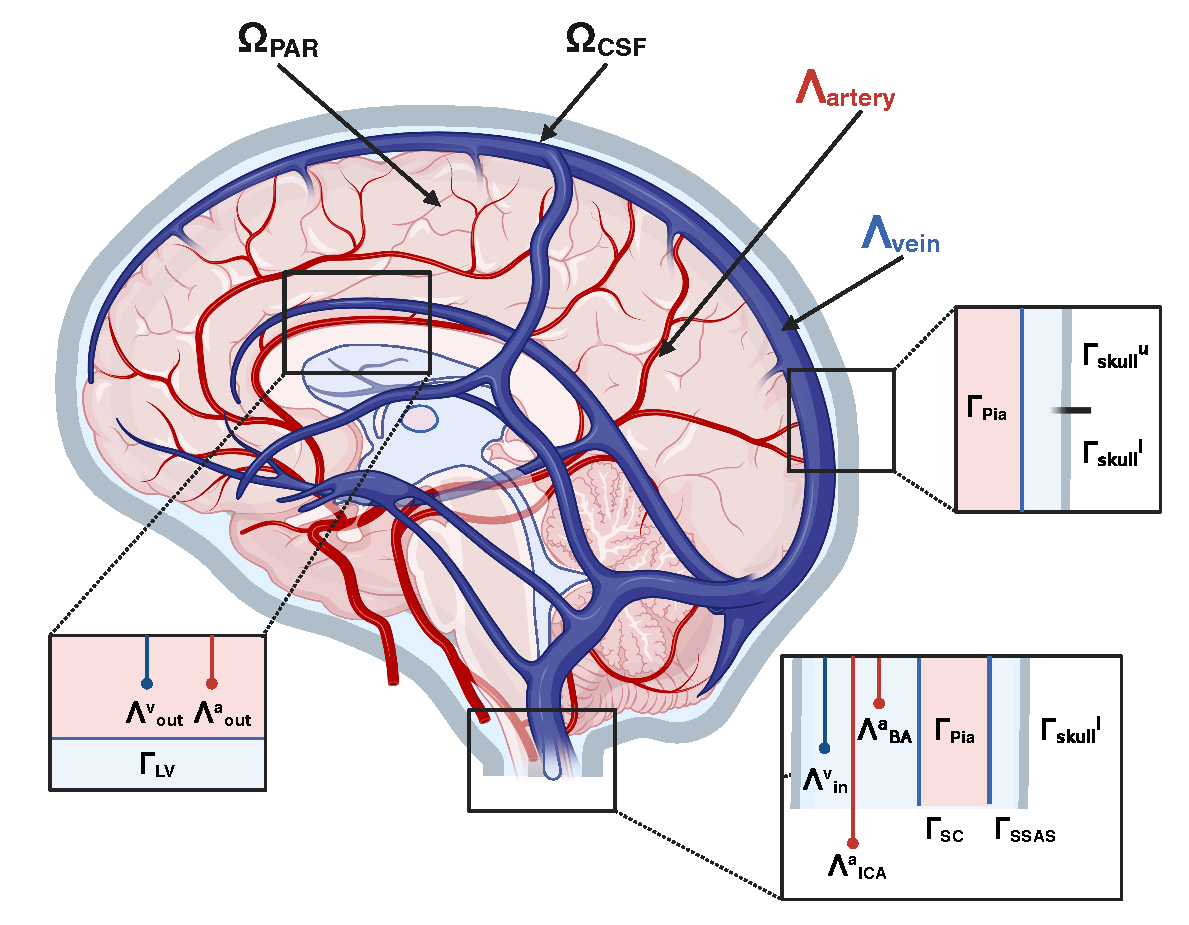
\includegraphics[width=\textwidth]{figures/Brain-PVS-callouts.pdf}
%%          \label{fig:intracranial_domains}
%%      \end{subfigure}
%%      \hfill
%%      \begin{subfigure}[b]{0.3\textwidth}
%%          \centering
%%          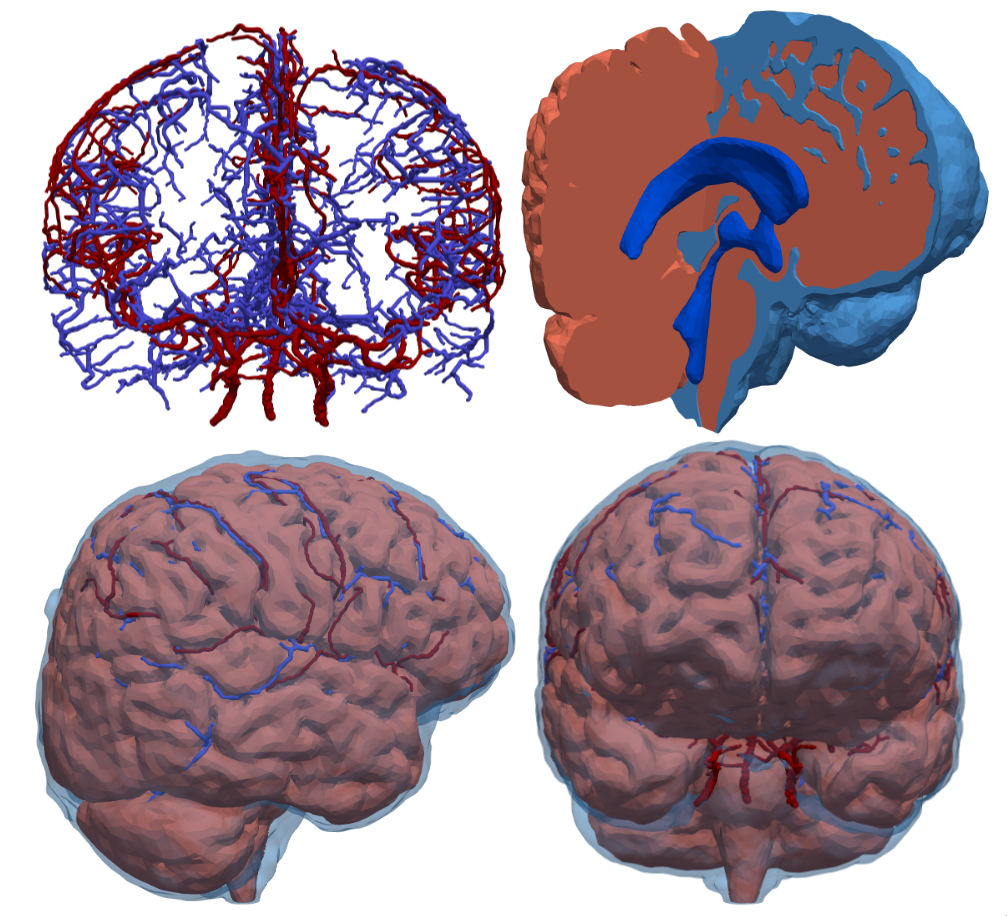
\includegraphics[width=\textwidth]{figures/geometry_concept.png}
%%          \caption{The arterial (red) and venous (blue) networks (top left), the parenchyma and CSF space (top right), combined (bottom row)}
%%          \label{fig:three sin x}
%%      \end{subfigure}
%%      \hfill
%%      \begin{subfigure}[b]{0.24\textwidth}
%%          \centering
%%          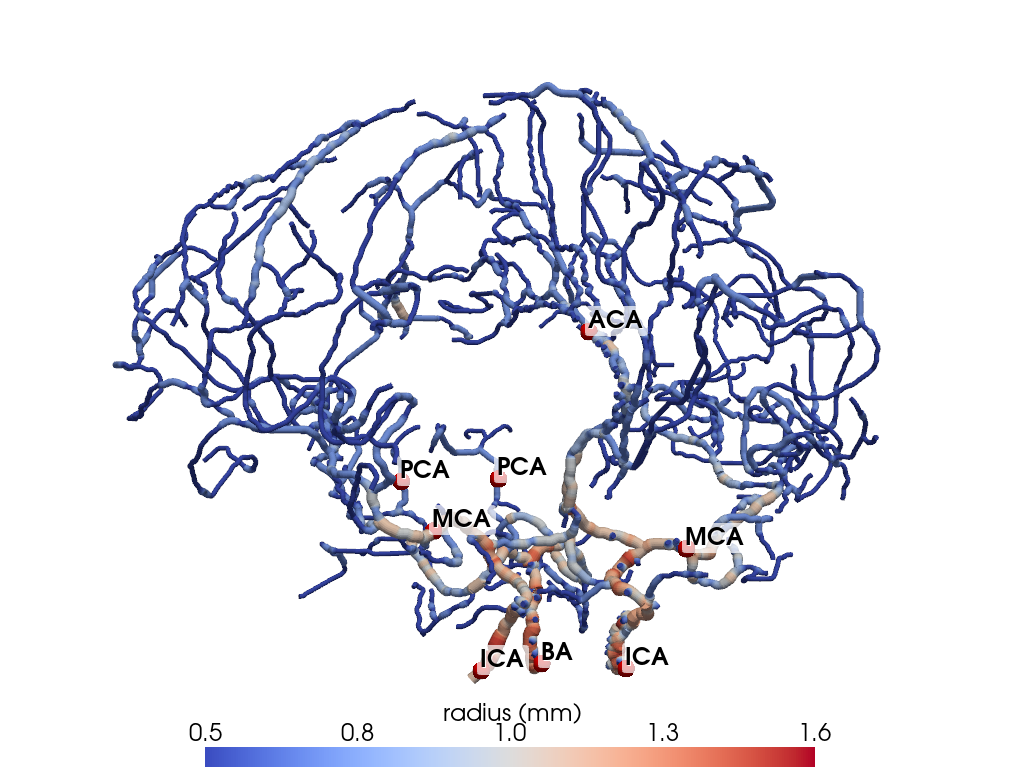
\includegraphics[trim={4cm 0 4cm 0},clip,width=\textwidth]{figures/labeled_arteries.png}
%%          \caption{The arterial network with the main cerebral arteries: internal carotid artery (ICA), middle cerebral artery (MCA), anterior cerebral artery (ACA) and posterior cerebral artery (PCA)}
%%          \label{fig:five over x}
%%      \end{subfigure}
%%      %\caption{@Marius: Starts adding parts of this. \mer{MER: Concept figure illustrating the compartments and story line. (A) Concept sketch of the SAS, PVS and the brain; (B) Visualization of geometry domains (brain, sas and vasculature; think about colors and associations; please don't make blood blue and water red e.g.) ; (C) Zoom-in/detail on vasculature, which are which arteries (ACA, MCA, PCA, CoW)  and veins (XXX); (D) Zoom-in 2 on vascular position versus SAS and brain; (E) Zoom-in 3 on where PVS ends; (F) Illustration of boundaries? (G) Concept illustration of the mathematical model (diffusion, convection, exchange, boundaries).}}
%% \label{fig:concept}
%% \end{figure}


\begin{table}
\begin{center}
  \begin{tabular}{ll|llllll|ll}
    \toprule
    & Description & $R$ & $\xi_{\rm PVS-SAS}$, $\xi_{\rm PVS-PAR}$ & $\beta_{\rm efflux}$ & $D$ & $\hat{u}$ & $\mathbf{u}_{\rm SAS, PAR}$ & $g_{\rm influx}$ & $c_0$ \\
    \midrule
    A & Baseline  & $R_2 = 2 R_1$ & $\xi$, $\tilde \xi$\cite{koch2023estimates} &  $10^{-4}$ mm$^2$/s\cite{hornkjol2022csf} & $D^{\rm gad}$\cite{sykova2008diffusion, valnes2020apparent}  & $\hat{u} = \hat{u}_{\rm prod}$ & $\mathbf{u}_{\rm SAS} = \mathbf{u}_{\rm prod}$, $\mathbf{u}_{\rm PAR} = 0$ & $> 0$ & 0 \\
    B & PVS "sheaths" & $R_2 = 2 R_1$ & $0, 0.5 \xi, \xi, 2 \xi, 1000 \xi \approx \infty$, --\cite{koch2023estimates} & -- & --  &  --  & --  & -- & -- \\
    C & Larger PVS & $R_2 = N R_1$ & -- & -- & --  &  --  & -- & -- & -- \\
    D & PVS I & $R_2 = 2 R_1$ & $\xi$, -- & -- & --  &  $\hat{u} = \hat{u}_{\rm prod} + \uparrow$  & -- & -- & -- \\
    E & PVS II & $R_2 = 2 R_1$ & $\xi$, -- & -- & --  &  $\hat{u} = \hat{u}_{\rm prod} + \uparrow\uparrow$  & -- & -- & -- \\
    F & PVS III & $R_2 = 2 R_1$ & $\xi$, -- & -- & $10 D_{\rm PVS}$ &  $\hat{u} = \hat{u}_{\rm prod}$  & -- & -- & -- \\
    G & Glymphatics & $R_2 = 2 R_1$ & $\xi$, -- & -- & \cite{sykova2008diffusion, valnes2020apparent} &  $\hat{u} = \hat{u}_{\rm prod} + \uparrow$  & $\mathbf{u}_{\rm PAR}$ > 0 & -- & -- \\
    H & Sleep &  &  & &  &  &  & & \\
    I & Pathology I &  &  & &  &  &  & & \\
    J & Pathology II &  &  & &  &  &  & & \\
    \midrule
    X & Clearance & $R_2 = 2 R_1$ & $50\%$, $\xi$ & -- & $D^{\rm gad, \tau, A\beta}$  &  $\hat{u} = \hat{u}_{\rm prod}$  & -- & $0$ & $1$ \\
    Y & (PVS) & $R_2 = 2 R_1$ & $50\%$, $\xi$ & -- & $D^{\rm gad, \tau, A\beta}$  &  $\hat{u} = \hat{u}_{\rm prod} + \uparrow$  & -- & -- & -- \\
    Z & (Glymphatic) & $R_2 = 2 R_1$ & $50\%$, $\xi$ & -- & $D^{\rm gad, \tau, A\beta}$  &  $\hat{u} = \hat{u}_{\rm prod} + \uparrow$  & $\mathbf{u}_{\rm PAR}$ > 0 & -- & -- \\
    \bottomrule
    \end{tabular}
    \end{center}
\caption{Overview of models (-- denotes as immediately above). Model A represents a baseline scenario with semi-permeable barriers between the PVS and SAS ($\xi_{\rm PVS-SAS} \approx 50\%$, \mer{we try to estimate this value by a bit of trial-and-error from the observations of timings of PVS-SAS and SAS from~\cite{eide2024functional}})~\cite{bedussi2017paravascular} and astrocytic endfeet forming barriers within the parenchyma~\cite{koch2023estimates}. $R_1$ and $R_2$ denotes the inner and outer radius of the PVS, with PVS width comparable to vascular diameter ($R_2 - R_1 \approx 2 R_1$)\cite{mestre2018flow} as a baseline. The extracranial solute efflux permeability $\beta_{\rm efflux}$ is uniformly distributed over the outer SAS boundary with a reasonable rate as baseline\cite{hornkjol2022csf, eide2021clinical, ringstad2024glymphatic}. At baseline, the effective diffusion coefficients $D^{\rm x}_{\rm SAS} = D^{\rm x}_{\rm PVS}$ of the SAS and PVS represent the free diffusion coefficient of Gadubutrol (${\rm x} = {\rm gad}$) in CSF (water), and $D^{\rm x}_{\rm PAR}$ the effective diffusion coefficient of human cortical tissue, all at body temperature. At baseline, we consider net flow due to CSF-production in the SAS (and PVS): $\mathbf{u}_{\rm SAS} > 0$ (and $\hat{u} > 0$), but no additional effects from perivascular pulsatility nor bulk flow in the parenchyma $\mathbf{u}_{\rm PAR} = 0$. Due to the timescale for human intracranial tracer transport (minutes to hours) compared to typical (cardiac, respiratory, slow vasomotion) human intracranial pulsatility (0.1 -- 1 Hz), we consider net (constant-in-time) flow fields only in subsequent model variations. Model B represents a PVS-SAS interface configuration with minimal or more permeable structural barriers~\cite{eide2024functional}, while Model C represents enlarged PVS. Models D, E, and F represent three perivascular pathway scenarios with more rapid flow in the PVS induced by vasomotion (PVS I)~\cite{gjerde2023directional} or a net fluid source in the PVS (1D Stokes flow)/net pressure difference between PVS inlets and outlets (PVS II), or with enhanced effective diffusion due to mixing (PVS III)~\cite{hornkjol2022csf, troyetsky2021dispersion, vinje2023human}, respectively. Model G attempts to represent a glymphatic--like convective flow within the parenchyma. \mer{Ideas could be:  (a) network induces arterial and venous sources in a Darcy porous media flow model (reflects the glymphatic hypothesis), (b) Croci-style \cite{croci2019uncertainty}, (c) \cite{vinje2023human}} Model H represents physiological alterations associated with sleep (lower CSF production, enhanced diffusion within the parenchyma, enhanced PVS pulsatility), while Models I--J represents variations associated with pathologies (e.g.~dementia, hypertension, angiopathies, CSF-disorders and/or others). Models X--Z represent version of the aforementioned scenarios but for studying metabolite clearance (instead of solute influx).}
\label{tab:scenarios}
\end{table}
